\documentclass[12pt]{article}

\pagestyle{empty}
\setlength{\topmargin}{0in}
\setlength{\headheight}{0in}
\setlength{\topsep}{0in}
\setlength{\textheight}{9in}
\setlength{\oddsidemargin}{0in}
\setlength{\evensidemargin}{0in}
\setlength{\textwidth}{6.5in}

\usepackage{palatino,graphics,amsmath,amssymb,enumitem}

\newcommand{\ds}{\displaystyle}
\newcommand{\vs}[1]{\vspace{#1in}}
\renewcommand{\vss}[1]{\vspace*{#1in}}
\newcommand{\bvec}{{\mathbf b}}
\newcommand{\cvec}{{\mathbf c}}
\newcommand{\dvec}{{\mathbf d}}
\newcommand{\evec}{{\mathbf e}}
\newcommand{\fvec}{{\mathbf f}}
\newcommand{\qvec}{{\mathbf q}}
\newcommand{\uvec}{{\mathbf u}}
\newcommand{\vvec}{{\mathbf v}}
\newcommand{\wvec}{{\mathbf w}}
\newcommand{\xvec}{{\mathbf x}}
\newcommand{\yvec}{{\mathbf y}}
\newcommand{\zvec}{{\mathbf y}}
\newcommand{\zerovec}{{\mathbf 0}}
\newcommand{\real}{{\mathbb R}}
\newcommand{\twovec}[2]{\left[\begin{array}{r}#1 \\ #2
    \end{array}\right]}
\newcommand{\ctwovec}[2]{\left[\begin{array}{c}#1 \\ #2
   \end{array}\right]}
\newcommand{\threevec}[3]{\left[\begin{array}{r}#1 \\ #2 \\ #3
  \end{array}\right]}
\newcommand{\cthreevec}[3]{\left[\begin{array}{c}#1 \\ #2 \\ #3
    \end{array}\right]}
\newcommand{\fourvec}[4]{\left[\begin{array}{r}#1 \\ #2 \\ #3 \\ #4
    \end{array}\right]}
\newcommand{\cfourvec}[4]{\left[\begin{array}{c}#1 \\ #2 \\ #3 \\ #4
    \end{array}\right]}
\newcommand{\mattwo}[4]{\left[\begin{array}{rr}#1 & #2 \\ #3 & #4 \\ \end{array}\right]}
\renewcommand{\span}[1]{\text{Span}\{#1\}}
\newcommand{\bcal}{{\cal B}}
\newcommand{\ccal}{{\cal C}}
\newcommand{\scal}{{\cal S}}
\newcommand{\wcal}{{\cal W}}
\newcommand{\ecal}{{\cal E}}
\newcommand{\coords}[2]{\left\{#1\right\}_{#2}}
\newcommand{\gray}[1]{\color{gray}{#1}}
\newcommand{\lgray}[1]{\color{lightgray}{#1}}
\newcommand{\rank}{\text{rank}}
\newcommand{\col}{\text{Col}}
\newcommand{\nul}{\text{Nul}}

\begin{document}

\noindent
{\bf Mathematics 227} \\ 
{\bf Review}

\bigskip
\begin{enumerate}
\item
  \begin{enumerate}[label=(\alph*)]
  \item What does it mean for a set of vectors to be linearly
    dependent?
    
    \vs{1}
  \item Is the following set of vectors linearly dependent?
    
    $$
    \vvec_1=\fourvec2{-1}31,\hspace*{24pt}
    \vvec_2=\fourvec12{-1}1,\hspace*{24pt}
    \vvec_3=\fourvec0{-5}5{-1},\hspace*{24pt}
    \vvec_4=\fourvec0123.
    $$
    
    \vs{1}
  \item If so, find one vector that is a linear combination of the
    others.
    
    \vs{1}
  \item Explain why the columns of a matrix are linearly dependent
    if the matrix has a column without a pivot.
    
    \vs{1}
  \end{enumerate}

\item Suppose that people either live in urban or rural areas and that
  every year, 
  \begin{itemize}
  \item 97\% of people living in urban areas remain in urban areas,
    and
  \item 95\% of people living in rural areas remain in rural areas.
  \end{itemize}

  Let $\xvec=\twovec UR$ be the vector describing the fraction of
  people $U$ living in urban areas and the fraction of people $R$
  living in rural areas in one year.  The matrix transformation
  $T:\real^2\to\real^2$ describes the fractions the next year.

  \medskip
  Find a matrix $A$ that represents the matrix transformation.

  \vs{1}
  Suppose that in 2010, 60\% of the population lived in urban areas
  and 40\% in rural areas.  How are the populations distributed in
  2011.

  \vs{1}
  How were the populations distributed in 2009?

  \vs{1}
  How are the populations distributed in 2018?

  \vs{1}
\item Find the matrix that reflects vectors in the plane across the
  line $y=-x$.

  \vs{1}
  Find the matrix that rotates vectors by 90$^\circ$ in the clockwise
  direction.

  \vs{1}
  What geometric operation is performed if we first reflect in the
  line $y=-x$ and then rotate by 90$^\circ$ in the clockwise
  direction?

  \vs{1}
\item Suppose that $A$ is an invertible $n\times n$ matrix.  Explain
  why the columns of $A$ form a basis for $\real^n$.

  \vs{1}
  Suppose that
  $
  A =
  \left[
    \begin{array}{rrr}
      3 & 1 & -1 \\
      2 & 2 & 1 \\
      -1 & 2 & 3
    \end{array}
  \right].
  $
  Explain how you know that $A$ is invertible?

  \vs{1}
  Explain an algorithm for finding $A^{-1}$.

  \vs{1}
  Find the solution to the equation $A\xvec = \threevec2{-5}{10}$
  using the inverse of $A$.

  \vs{1}
  Suppose that $A$ and $B$ are both $2\times2$ invertible matrices and
  that
  $$
  A^{-1} =
  \left[
    \begin{array}{cc}
      2 & 1 \\
      -1 & -1 \\
    \end{array}
  \right],\hspace*{24pt}
  B^{-1} =
  \left[
    \begin{array}{cc}
      1 & 3 \\
      0 & -1 \\
    \end{array}
  \right].
  $$
  Without finding $A$ and $B$, find the solution to the equation
  $BA\xvec = \twovec3{-2}$. 

  \vs{1}
\item Suppose that $\vvec_1$ and $\vvec_2$, the vectors shown
  below, form a basis $\bcal$.

  \begin{center}
    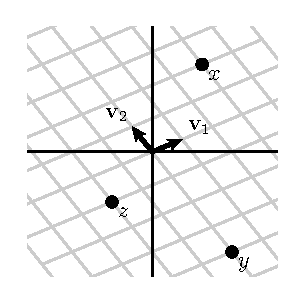
\includegraphics{21-linear-comb.eps}
  \end{center}

  Indicate the vector $\wvec$ where
  $\coords{\wvec}{\bcal}=\twovec{-2}2$.

  \vs{0.2}
  Find

  \medskip
  $\bullet \coords{\vvec_1}{\bcal}$

  \medskip
  $\bullet \coords{\xvec}{\bcal}$

  \medskip
  $\bullet \coords{\yvec}{\bcal}$

  \medskip
  $\bullet \coords{\zvec}{\bcal}$

\item Suppose that
  $$
  \vvec_1=\threevec{-4}7{-6},\hspace*{24pt}
  \vvec_2=\threevec{5}{-8}{7},\hspace*{24pt}
  \vvec_3=\threevec{-3}5{-4}.
  $$
  Explain why $\vvec_1$, $\vvec_2$, and $\vvec_3$ form a basis $\bcal$
  for $\real^3$.

  \vs{1}
  Find the coordinate representations $\coords{\evec_1}{\bcal}$ and
  $\coords{\evec_2}{\bcal}$.

  \vs{1}
  If $\coords{\xvec}{\bcal}=\threevec2{-1}3$, find $\xvec$.
  


  
    
    


\end{enumerate}


\end{document}
